\documentclass[11pt,a4paper]{report}
\usepackage[margin=1in]{geometry}
\usepackage[T1]{fontenc}
\usepackage{lmodern}
\usepackage{hyperref}
\usepackage{booktabs}
\usepackage{longtable}
\usepackage{listings}
\usepackage{xcolor}
\usepackage{graphicx}
\usepackage{tikz}
\usetikzlibrary{shapes,arrows.meta,positioning,fit}

\hypersetup{colorlinks=true,linkcolor=blue,urlcolor=blue}

\lstdefinestyle{bash}{
  basicstyle=\ttfamily\small,
  breaklines=true,
  frame=single,
  backgroundcolor=\color{gray!8}
}

\title{CXR OpenTelemetry Lab Manual\\
\large SW.11 --- Starter milestone \#7\\
\large Connecting rehearsal :8251 to Jaeger}
\author{CXR Ops Lab --- \texttt{cxr-ops-lab}}
\date{2026-05-31}

\begin{document}
\maketitle
\begin{abstract}
Step-by-step lab for \textbf{OpenTelemetry (SW.11)}: how \textbf{cxr-ui-rehearsal} on
\textbf{:8251} sends traces to the OTel Collector and how \textbf{Jaeger UI (:16686)} shows them
when you click \textbf{Run Analysis} in Claim Studio. The collector has \textbf{no web UI}; Jaeger is the viewer.
Use this PDF as the implementation record for traces vs metrics (Prometheus/Grafana).
\end{abstract}
\tableofcontents
\newpage

\chapter{Where you view telemetry}

\begin{center}
\begin{tabular}{llll}
\toprule
Signal & Tool & URL & Web UI? \\
\midrule
Metrics & Prometheus & :9090 & Yes \\
Dashboards & Grafana & :3001 & Yes \\
\textbf{Traces} & \textbf{Jaeger} & \textbf{:16686} & \textbf{Yes --- use this} \\
OTLP ingest & OTel Collector & :4318 & \textbf{No} (API only) \\
\bottomrule
\end{tabular}
\end{center}

\noindent\textbf{Key point:} Opening \url{http://localhost:4318} in a browser often returns 404 --- that is normal.
The collector runs in the background. You only \emph{see} trace data in \textbf{Jaeger}.

\chapter{How :8251 connects to Jaeger (highlight)}

This chapter documents the connection you verified: \textbf{Run Analysis} on Claim Studio
and traces appearing in Jaeger within seconds.

\section{End-to-end path}

\begin{center}
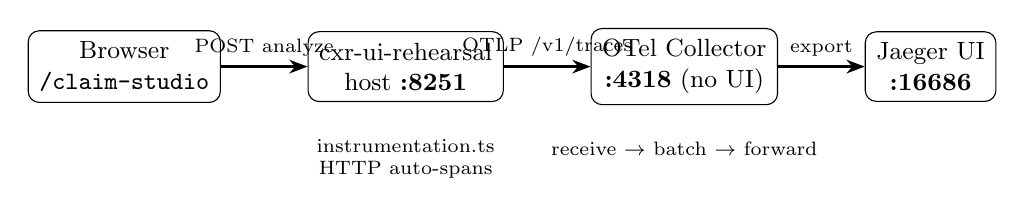
\begin{tikzpicture}[
  node distance=0.65cm and 0.5cm,
  box/.style={draw, rounded corners, minimum height=0.75cm, align=center, font=\small, inner sep=4pt},
  arr/.style={-{Stealth}, thick}
]
  \node[box] (br) {Browser\\\texttt{/claim-studio}};
  \node[box, right=1.1cm of br] (ui) {cxr-ui-rehearsal\\host \textbf{:8251}};
  \node[box, right=1.1cm of ui] (col) {OTel Collector\\\textbf{:4318} (no UI)};
  \node[box, right=1.1cm of col] (jui) {Jaeger UI\\\textbf{:16686}};
  \draw[arr] (br) -- node[above,font=\scriptsize]{POST analyze} (ui);
  \draw[arr] (ui) -- node[above,font=\scriptsize]{OTLP /v1/traces} (col);
  \draw[arr] (col) -- node[above,font=\scriptsize]{export} (jui);
  \node[below=0.35cm of ui, font=\scriptsize, align=center] {instrumentation.ts\\HTTP auto-spans};
  \node[below=0.35cm of col, font=\scriptsize, align=center] {receive $\rightarrow$ batch $\rightarrow$ forward};
\end{tikzpicture}
\end{center}

\section{What ``connects'' the rehearsal app}

\begin{enumerate}
  \item \textbf{Observe stack running} --- \texttt{./scripts/07-observe-up.sh} starts collector + Jaeger on Docker network \texttt{cxr\_observe}.
  \item \textbf{Environment variables on the :8251 process} (must be set \emph{before} \texttt{next dev}):
  \begin{lstlisting}[style=bash]
export OTEL_EXPORTER_OTLP_ENDPOINT=http://127.0.0.1:4318
export OTEL_SERVICE_NAME=cxr-ui-rehearsal
  \end{lstlisting}
  Template: \texttt{cxr-ops-lab/.env.otel.example}.
  \item \textbf{Next.js instrumentation hook} --- \texttt{instrumentation.ts} calls \texttt{register()} at Node process start;
  loads \texttt{instrumentation/register-otel-node.ts} (NodeSDK + OTLP HTTP exporter + HTTP auto-instrumentation).
  If \texttt{OTEL\_EXPORTER\_OTLP\_ENDPOINT} is unset, tracing is off (normal systemd :8251).
  \item \textbf{User action} --- \textbf{Run Analysis} sends \texttt{POST /api/claim-studio/analyze}.
  OTel records spans on the Node server and exports them to the collector.
  \item \textbf{Jaeger UI} --- Search $\rightarrow$ Service \texttt{cxr-ui-rehearsal} $\rightarrow$ new \textbf{POST} trace (often 5--11\,s duration).
\end{enumerate}

\section{Why Run Analysis appeared in Jaeger immediately}

\begin{itemize}
  \item The browser POST hits the same Next.js process you started with \texttt{OTEL\_*} set.
  \item HTTP instrumentation creates a trace for that request (not for the whole browser session).
  \item Spans are sent to \texttt{http://127.0.0.1:4318/v1/traces}, then forwarded to Jaeger.
  \item Jaeger Search lists the trace under service \texttt{cxr-ui-rehearsal}.
  \item Waterfall typically shows \texttt{executing api route} for most of the duration (Python analyzer subprocess is \emph{not} a separate span in this bootcamp scope).
\end{itemize}

\section{GET vs POST traces (why the list is ``divided'')}

\begin{center}
\begin{tabular}{lll}
\toprule
HTTP & When & Typical duration \\
\midrule
GET & Page loads, navigation & ms -- 2\,s \\
POST & \textbf{Run Analysis} & $\sim$5--11\,s \\
\bottomrule
\end{tabular}
\end{center}
Jaeger shows \textbf{one trace per HTTP request}. Several GETs plus one or more POSTs = multiple rows in Search.

\section{systemd vs manual dev (:8251)}

The user unit \texttt{cxr-rehearsal-dev} serves daily dev on :8251 \textbf{without} \texttt{OTEL\_*}.
For SW.11:
\begin{lstlisting}[style=bash]
systemctl --user stop cxr-rehearsal-dev
export OTEL_EXPORTER_OTLP_ENDPOINT=http://127.0.0.1:4318
export OTEL_SERVICE_NAME=cxr-ui-rehearsal
cd cxr-ui-prune-rehearsal/cxr-ui
npm run dev:rehearsal
\end{lstlisting}
After the lab: \texttt{systemctl --user start cxr-rehearsal-dev} for normal untraced dev.

\chapter{Step-by-step procedure}

\section{Step 1 --- Start observe + OTel stack}
\begin{lstlisting}[style=bash]
cd cxr-ops-lab
./scripts/07-observe-up.sh
./scripts/11-otel-smoke.sh
\end{lstlisting}
Open \url{http://localhost:16686} (Jaeger UI only).

\section{Step 2 --- Install npm packages (once)}
\begin{lstlisting}[style=bash]
cd cxr-ui-prune-rehearsal/cxr-ui
npm install
\end{lstlisting}

\section{Step 3 --- Wire :8251 (env + dev server)}
Stop conflicting :8251 service; export OTel env; start rehearsal dev (see Chapter 2).

\section{Step 4 --- Golden path: Run Analysis $\rightarrow$ Jaeger}
\begin{enumerate}
  \item \url{http://localhost:8251/claim-studio}
  \item Click \textbf{Run Analysis}; confirm \texttt{POST /api/claim-studio/analyze} returns 200.
  \item \url{http://localhost:16686} $\rightarrow$ Search $\rightarrow$ Service \texttt{cxr-ui-rehearsal} $\rightarrow$ Find Traces.
  \item Open newest \textbf{POST} trace; screenshot search + waterfall for evidence.
\end{enumerate}
Success criterion: POST trace visible right after Run Analysis --- that proves :8251 is connected to Jaeger.

\section{Step 5 --- Write evidence note}
Edit \texttt{evidence/SW11-otel-verify-2026-05-29.md}:
\begin{itemize}
  \item Document :8251 + \texttt{OTEL\_*} $\rightarrow$ :4318 $\rightarrow$ Jaeger connection.
  \item Spans start: \texttt{instrumentation.ts}, HTTP auto-instrumentation.
  \item Not traced yet: Python \texttt{spawn} subprocess.
  \item Attach PNGs (e.g.\ \texttt{SW11-jaeger-search-*.png}, \texttt{SW11-jaeger-waterfall-post-analyze-*.png}).
\end{itemize}

\chapter{Implementation checklist (repeat on another machine)}

\begin{enumerate}
  \item Start collector + Jaeger (\texttt{07-observe-up.sh}).
  \item Set \texttt{OTEL\_EXPORTER\_OTLP\_ENDPOINT} and \texttt{OTEL\_SERVICE\_NAME} before starting Next.
  \item Ensure \texttt{instrumentation.ts} + \texttt{register-otel-node.ts} in the app; \texttt{next.config.ts} lists OTel in \texttt{serverExternalPackages}.
  \item Generate traffic (Run Analysis).
  \item Verify only in Jaeger :16686 (not :4318).
\end{enumerate}

\chapter{Optional: Compose :3000}

Rebuild \texttt{cxr-ui:compose} after OTel packages are in the image context, then:
\begin{lstlisting}[style=bash]
./scripts/07-observe-up.sh
docker compose -f compose.yaml -f compose.host.yaml \
  -f compose.otel-link.yaml up -d
\end{lstlisting}
Jaeger service name: \texttt{cxr-ui-compose}.

\chapter{File reference}

\begin{longtable}{@{}p{4.4cm}p{8.6cm}@{}}
\toprule
File & Purpose \\
\midrule
\endhead
\texttt{compose.observe.yaml} & Prometheus, Grafana, Jaeger, collector \\
\texttt{observe/otel-collector-config.yaml} & OTLP in $\rightarrow$ Jaeger out \\
\texttt{instrumentation.ts} & Next.js register hook (edge-safe entry) \\
\texttt{instrumentation/register-otel-node.ts} & NodeSDK + OTLP + shutdown handlers \\
\texttt{.env.otel.example} & Env template for :8251 / :3000 \\
\texttt{compose.otel-link.yaml} & Compose network link to collector \\
\texttt{scripts/11-otel-smoke.sh} & Health probe \\
\bottomrule
\end{longtable}

\chapter{Troubleshooting}

\begin{itemize}
  \item \textbf{No traces} --- OTel env must be set \emph{before} \texttt{next dev}; restart dev after exporting vars.
  \item \textbf{Analyze works, Jaeger empty} --- Filter Service = \texttt{cxr-ui-rehearsal}; generate traffic after server start.
  \item \textbf{:4318 browser 404} --- Expected; use Jaeger :16686.
  \item \textbf{Port 8251 busy} --- Stop \texttt{cxr-rehearsal-dev} or old dev process.
  \item \textbf{Disable OTel} --- \texttt{export OTEL\_SDK\_DISABLED=true}.
\end{itemize}

\chapter{Study plan linkage}

\begin{center}
\begin{tabular}{ll}
\toprule
Item & Maps to \\
\midrule
Starter milestone \#7 & SW.11 \\
Module 1 step M1.6 & OTel concepts + C4 telemetry edge \\
After this lab & SW.12--SW.18 electives \\
\bottomrule
\end{tabular}
\end{center}

\chapter{Live adjustments (made traces work on :8251)}

\begin{itemize}
  \item \textbf{Next.js 16 \texttt{searchParams}} --- \texttt{app/page.tsx}: \texttt{await Promise.resolve(searchParams)} (fixes runtime error on \texttt{/}).
  \item \textbf{Instrumentation split} --- \texttt{instrumentation.ts} = thin Edge-safe hook; \texttt{instrumentation/register-otel-node.ts} = NodeSDK, OTLP exporter, \texttt{process.on} shutdown (avoids Edge warnings).
  \item \textbf{Resource API} --- \texttt{new Resource(\{...\})} instead of deprecated \texttt{resourceFromAttributes}.
  \item \textbf{\texttt{next.config.ts}} --- \texttt{serverExternalPackages} lists OTel packages for Next bundler.
  \item \textbf{:8251 ownership} --- \texttt{systemctl --user stop cxr-rehearsal-dev} before \texttt{OTEL_*} + \texttt{npm run dev:rehearsal}; env must be set \emph{before} dev start.
  \item \textbf{:4318 browser 404} --- expected; only Jaeger :16686 is the trace UI.
\end{itemize}

\chapter{UI evidence --- Jaeger (:16686)}

Verified after Claim Studio \textbf{Run Analysis} on \textbf{:8251} with \texttt{OTEL\_EXPORTER\_OTLP\_ENDPOINT=http://127.0.0.1:4318}.

\begin{figure}[htbp]
\centering
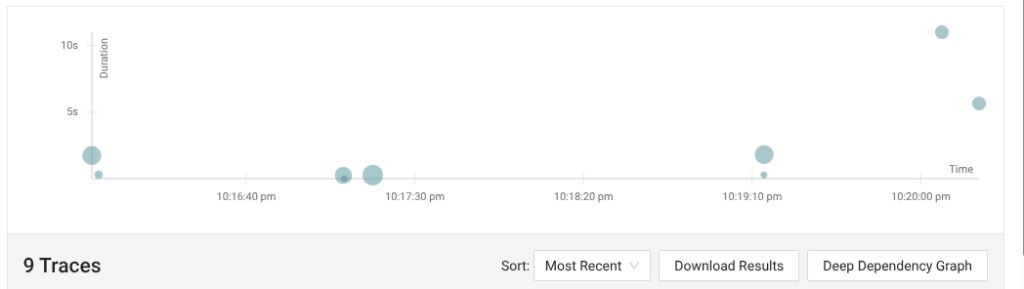
\includegraphics[width=0.92\textwidth]{../evidence/SW11-jaeger-search-2026-05-30.png}
\caption{Jaeger Search --- service \texttt{cxr-ui-rehearsal}; POST analyze traces visible.}
\end{figure}

\begin{figure}[htbp]
\centering
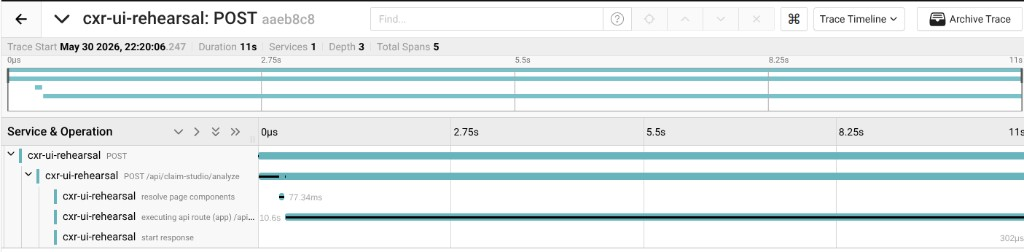
\includegraphics[width=0.92\textwidth]{../evidence/SW11-jaeger-waterfall-post-analyze-2026-05-30.png}
\caption{Waterfall for POST \texttt{/api/claim-studio/analyze} (${\sim}$5--11\,s).}
\end{figure}

\end{document}
